\documentclass[12pt,a4paper]{article}

\usepackage{epcc}
\usepackage{graphicx}
\usepackage{listings}
\usepackage{color}
\usepackage{amsmath}
\usepackage{tikz}
\usepackage{makecell}
\usepackage{array}
\usepackage{wrapfig}
\usepackage{multirow}
\usepackage{tabu}
\usepackage{realboxes}

\definecolor{mygreen}{rgb}{0,0.6,0}
\definecolor{mygray}{rgb}{0.5,0.5,0.5}
\definecolor{mymauve}{rgb}{0.58,0,0.82}

\lstset{ 
	backgroundcolor=\color{white},   % choose the background color; you must add \usepackage{color} or \usepackage{xcolor}; should come as last argument
	basicstyle=\footnotesize,        % the size of the fonts that are used for the code
	breakatwhitespace=false,         % sets if automatic breaks should only happen at whitespace
	breaklines=true,                 % sets automatic line breaking
	captionpos=b,                    % sets the caption-position to bottom
	commentstyle=\color{mygreen},    % comment style
	deletekeywords={...},            % if you want to delete keywords from the given language
	escapeinside={\%*}{*)},          % if you want to add LaTeX within your code
	extendedchars=true,              % lets you use non-ASCII characters; for 8-bits encodings only, does not work with UTF-8
	frame=none,	                   % adds a frame around the code
	keepspaces=true,                 % keeps spaces in text, useful for keeping indentation of code (possibly needs columns=flexible)
	keywordstyle=\color{blue},       % keyword style
	language=C,                 	 % the language of the code
	morekeywords={*,...},            % if you want to add more keywords to the set
	numbers=left,                    % where to put the line-numbers; possible values are (none, left, right)
	numbersep=5pt,                   % how far the line-numbers are from the code
	numberstyle=\tiny\color{mygray}, % the style that is used for the line-numbers
	rulecolor=\color{black},         % if not set, the frame-color may be changed on line-breaks within not-black text (e.g. comments (green here))
	showspaces=false,                % show spaces everywhere adding particular underscores; it overrides 'showstringspaces'
	showstringspaces=false,          % underline spaces within strings only
	showtabs=false,                  % show tabs within strings adding particular underscores
	stepnumber=5,                    % the step between two line-numbers. If it's 1, each line will be numbered
	stringstyle=\color{mymauve},     % string literal style
	tabsize=2,	                     % sets default tabsize to 2 spaces
	title=\lstname                   % show the filename of files included with \lstinputlisting; also try caption instead of title
}

\usepackage{hyperref}
\hypersetup{
	colorlinks=true, %set true if you want colored links
	linkcolor=black,  %choose some color if you want links to stand out
}

\newcommand{\sectionVspacing}{\vspace{15pt}} 


\begin{document}

\title{Threaded Programming Coursework Part 2}
\author{Exam number B136013}
\date{\today}

\makeEPCCtitle

\thispagestyle{empty}

\newpage
\clearpage

\tableofcontents

\newpage
\clearpage

\section{Introduction}

The goal of this coursework is to implement an alternative loop scheduling algorithm using OpenMP API. This method is called Affinity scheduling and it will be described in the following section.

\sectionVspacing

\section{Project Specification}
\subsection{Description}

In short, Affinity scheduling assigns a local set of iterations of the given loop to each thread. When each thread finishes these iterations it will search into the other threads, it will find the most loaded one and it will take a fraction of its workload. The algorithm will finish when all of the Local Sets has not more iterations to be done.

\subsection{Terminology}

In order to analyze the design, the definition of basic terminology is required. These terms are:

\begin{itemize}
  \item Chunk: A contiguous, non-empty subset of the iterations of a loop.
  \item Chunksize: The number of iterations for a specific Chunk.
  \item Local Set: A contiguous set of iterations assigned to each thread. In this case, the size of an initial Local Set is n/p, where n is the number of iterations for the running loop and p the number of threads.
  \item Most Loaded thread: At a specific time, the thread with the most remaining iterations of its given Local Set.
\end{itemize}

\sectionVspacing

\section{Design Analysis}

The scheduler has been designed with the necessary data structures and functions that hold vital information about the progress of the loop and each thread's workload. The functions containing the body of the loop has not been changed. The only modifications made are in runloop function providing the right Chunks for the loop.

\subsection{Initialization}
First and foremost, an OMP parallel region is created, with 2 shared variables. These variables are the loopid which determines which loop is running and a uninitialized pointer to Local\_Set\_Array, which will hold all the information for loop's progress. Then an initialization function is called that only one of the threads has to execute (first arrived thread). This function takes as input the number of iterations in the loop and the number of the active threads for this job to create a Local\_Set\_Array.

The Local\_Set\_Array is a C structure that contains an array of Local\_Set. Each thread can access a Local\_Set using a thread id as an index. For example, if we want to obtain the Local\_Set for thread number 4, the only thing we have to do is to look up for the fourth object in the array of Local\_Set\_Array structure. A Local\_Set in our implementation is a data structure containing:

\begin{itemize}
  \item The lowest position for the next to execute the Chunk
  \item The highest position for this Local Set
  \item An omp\_lock\_t that a thread is forced to obtain in order to update the Local\_Set
\end{itemize}

\subsection{Main Loop}
The main loop consists of 3 parts. The first one is the terminate condition. Each thread has to check if the loop has finished, in that case, each Local Set's lowest position equals the highest one. If yes then it exits and waits for the others to go to the finalization stage.

If this is not the case the thread tries to get the next Chunk. We define Chunk as a data structure that contains the lowest and highest positions that the thread has to run in the loop. The main interest of this project lies in the function that returns the next Chunk (more in the Synchronization section).

Once the thread has successfully obtained the new Chunk it calls the appropriate function to calculate the loop. This is where all of the loop calculations are done. The given parameters are the lowest and highest positions, which are contained in the next Chunk structure.

\subsection{Syncronization}
As mentioned before, synchronization is needed in the scheduler to obtain the next Chunk. In terms of correctness, the implementation of this function has to ensure that each iteration is going to run exactly one time by one thread. This means that the returned Chunks will contain a unique workload that has not been executed before. Also, for efficiency reasons race conditions between threads have to be reduced in a specific manner to avoid unnecessary stalls. OpenMP provides the omp\_lock\_t object. This allows as to gain exclusive access to a Local Set, in order to get correct Chunks.

The process to obtain the next Chunk is simple. In the beginning, a thread tries to acquire the next Chunk from its Local Set if this is successful it returns with the Chunk if not it has to steal workload for the most loaded thread.

To find the most loaded thread we have to iterate the array of Local Sets. Each time we lock the current Local Set and check its Chunksize. If its Chunksize is greater that the already locked we unlock the previous Local Set and continue the iteration.

Our most loaded Local Set remains locked to avoid any other threads trying to steal it from us. When the scan is completed and it is assured that the most loaded Local Set is taken, we update the indexes and then unlock it. By saying update, we mean that the lowest index is increased by the size of the new Chunksize. The new Chunksize is simply the remaining load of the Local Set divided by the number of threads. In this way, we guarantee that the selected Chunk is not executed by another thread. 

Waiting to obtain the lock for the next Local Set is unavoidable, but deadlocks are eliminated because no matter what happens each thread will eventually unlock the selected Local Set.

\subsubsection{Example}
Let's take the case in Figure \ref{diagram1} that 3 threads are running over 3 Local Sets. Threads 1 and 2 are getting Chunk from its Local Sets accordingly. Thread 3 has finished with Local Set 3 so it waits over Local Set 1 to lock it.\\

\begin{figure}[h!]
	\centering
	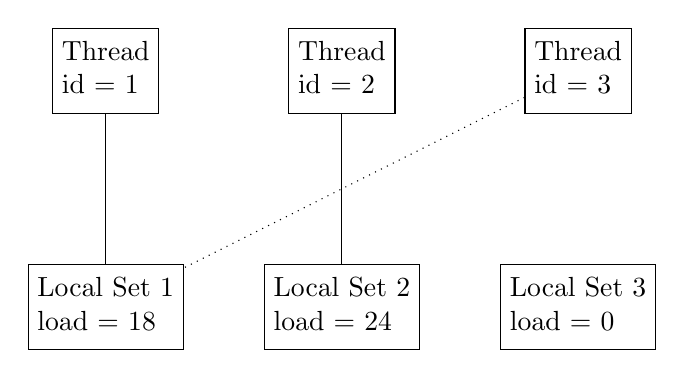
\begin{tikzpicture}
		\node[draw] at (0, 3)   (t1) {\makecell[l]{Thread\\id = 1}};
		\node[draw] at (3, 3)   (t2) {\makecell[l]{Thread\\id = 2}};
		\node[draw] at (6, 3)   (t3) {\makecell[l]{Thread\\id = 3}};
		
		\node[draw] at (0, 0)   (ls1) {\makecell[l]{Local Set 1\\load = 18}};
		\node[draw] at (3, 0)   (ls2) {\makecell[l]{Local Set 2\\load = 24}};
		\node[draw] at (6, 0)   (ls3) {\makecell[l]{Local Set 3\\load = 0}};
		
		\draw[solid] (t1) -- (ls1);
		\draw[solid] (t2) -- (ls2);
		\draw[dotted] (t3) -- (ls1);
	\end{tikzpicture}
	\caption{Stage 1} \label{diagram1}
\end{figure}


Once Thread 1 and 2 has unlocked its Local Sets, Thread 3 can lock Local Set 1 as the most loaded, based on Figure \ref{diagram2}.\\

According to Figure \ref{diagram3}, Thread 3 locks Local Set 2 and unlocks Local Set 1, because Local Set 2 is the most loaded until this point. In the meantime, while Thread 1 calculates its obtained Chunk from FIGURE 1, Thread 2 finished its caluclation and tries to lock Local Set 2. It has to wait until the Thread 3 unlocks it.\\
 
 \begin{figure}[h!]
 	\centering
 	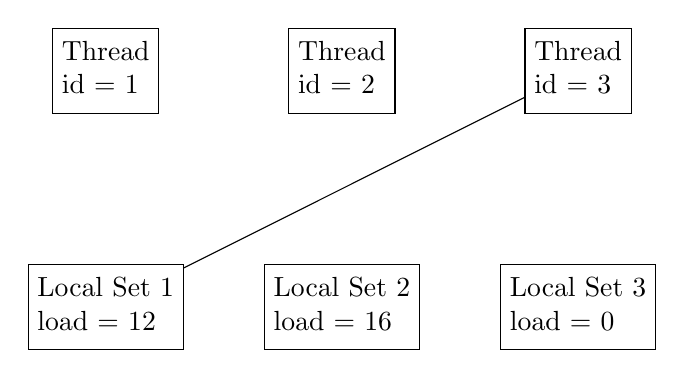
\begin{tikzpicture}
 	\node[draw] at (0, 3)   (t1) {\makecell[l]{Thread\\id = 1}};
 	\node[draw] at (3, 3)   (t2) {\makecell[l]{Thread\\id = 2}};
 	\node[draw] at (6, 3)   (t3) {\makecell[l]{Thread\\id = 3}};
 	
 	\node[draw] at (0, 0)   (ls1) {\makecell[l]{Local Set 1\\load = 12}};
 	\node[draw] at (3, 0)   (ls2) {\makecell[l]{Local Set 2\\load = 16}};
 	\node[draw] at (6, 0)   (ls3) {\makecell[l]{Local Set 3\\load = 0}};
 	
 	\draw[solid] (t3) -- (ls1);
 	\end{tikzpicture}
 	\caption{Stage 2} \label{diagram2}
 \end{figure}

 \begin{figure}[h!]
 	\centering
 	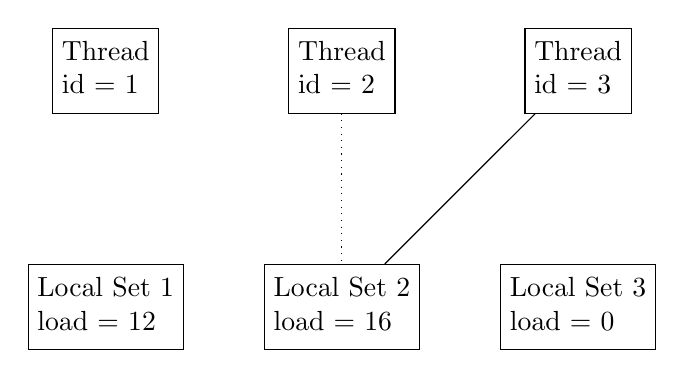
\begin{tikzpicture}
		\node[draw] at (0, 3)   (t1) {\makecell[l]{Thread\\id = 1}};
		\node[draw] at (3, 3)   (t2) {\makecell[l]{Thread\\id = 2}};
		\node[draw] at (6, 3)   (t3) {\makecell[l]{Thread\\id = 3}};
		
		\node[draw] at (0, 0)   (ls1) {\makecell[l]{Local Set 1\\load = 12}};
		\node[draw] at (3, 0)   (ls2) {\makecell[l]{Local Set 2\\load = 16}};
		\node[draw] at (6, 0)   (ls3) {\makecell[l]{Local Set 3\\load = 0}};
		
		\draw[dotted] (t2) -- (ls2);
		\draw[solid] (t3) -- (ls2);
 	\end{tikzpicture}
 	\caption{Stage 3} \label{diagram3}
 \end{figure}

This is an example that demonstrates when a Thread tries to steal workload from the others, if it Local Set has not remaining load.

\subsection{Finilization}
At the end of the loop, when every Local Set is empty, a function is called that is responsible to free the heap memory of the allocated Local\_Set\_Array. Just like the initialization phase, this method is called by the thread that arrives first in this section.

\clearpage

\section{Tools}

\subsection{Building}
The programming language used for the development of the scheduler is C. As regards the compiler we have used GCC from the GNU Compiler Collection including the -O3 option to ensure a high level of optimization in the sequential part of the problem. In terms of building, GNU Make rules made to compile, run and clean the project.

\subsection{Platform}
We have evaluated the scheduler running our experiments on the backend of Cirrus supercomputer using 1, 2, 4, 6, 8, 12 and 16 threads. Then, we compared our results with the best scheduling options that we found in coursework 1 (guided, 4 for Loop 1 and dynamic, 16 for Loop 2). The evaluation process includes graphs for each loop of the running time and the speedup against the number of threads. In addition, the speedup graphs contain the ideal speedup.

It worths mentioning that the measurements are a product of multiple runs over the loops, in order to reduce the noise in the timing results. To be more specific, the experiment has been executed 20 times for each thread configuration. This has been described in a Portable Batch System (PBS) script. Then the median values of each case have been used for the visual representations of the graphs.

To run the project in Cirrus execute
\begin{lstlisting}[language=bash]
  $ ./run.sh
\end{lstlisting}

This script will
\begin{itemize}
  \item Clean the the data/ and graphs/ folders
  \item Clean the executable and objective code
  \item Create the executable
  \item Submit the job to the backend of Cirrus
\end{itemize}

When the job is done run \Colorbox{mygray}{\lstinline|python check_correctness.py|} to check if the results. Following that, run \Colorbox{mygray}{\lstinline|python data_analyzer.py|} to analyze the exported data and create the appropriate graphs in the graphs/ folder.

\section{Evaluation}

\subsection{Loop 1}

\subsubsection{Running Time}

There is no denying the fact that running time for loop 1 is almost identical for guided, 4 and affinity scheduling options based on Figure \ref{runningTimeLoop1}.

\begin{figure}[h!]
	\centering
	\includegraphics[scale=0.6]{../graphs/loop1_running_time.eps}
	\caption{Running Time Loop 1}
	\label{runningTimeLoop1}
\end{figure}

At the beginning, let's take the case running with two threads. In Guided, 4 scheduling, the first thread is obliged to execute the first half of the iterations which is the heaviest workload. In contrast, in affinity scheduling, the first Local Set will be possibly executed by both of the threads. This happens because the second Local Set contains fewer calculations. Eventually, if we take into consideration the race conditions over the first Local Set we end up with one thread delaying the other. This communication overhead apparently results to the same execution time for both of the scheduling options.

As we increase the number of threads, on both occasions Chunksizes become smaller. We have multiple threads carrying the heavy work so communication is the only drawback. In both of the occasions, the heavy workload is distributed fairly among the thread. As a result, communication is the drawback. All of the threads in both of the scheduling options compete to take the next Chunk. The only difference that makes the guided, 4 scheduling a little bit faster is the minimum Chunksize. Guided, 4 obliges each thread to take at minumum 4 iterations to calculate. In contrary affinity scheduling has not such limitations which lead to the overall delay of affinity. Nevertheless, this behavior concludes to the similar running time between our cases.

At this point, we should point out that if the affinity scheduling had a way to define the minimum Chunksize, then the running time would have better results on the given problem.    

\subsubsection{Speedup}

When it comes to scalability, according to Figure \ref{speedupLoop1}, both of the scheduling options scale in simmilar manner. For 1 to 6 threads the speedup is extremely close to the ideal values. Beyond that point, in both cases the rate of changes is declined slightly until 12 threads.

In contrast, running on 16 threads the speedup results differ in each case. Guided, 4 option has better speedup. As mentioned before, this happens due to the fact that there is a limitation to the minimum Chunksize. If we take into consideration the fact that cache contains consecutive data because of the spatial locality, then guided, 4 works better as we increase the number of threads. This can become obvious for the last iterations. Guided, 4 could calculate 4 iterations much faster that affinity. As opposed to, affinity which will have to launch 4 threads to scan the Local Sets (including the race conditions) to acquire just on iteration and execute it.

\begin{figure}[h!]
    \centering
    \includegraphics[scale=0.6]{../graphs/loop1_speedup.eps}
    \caption{Speedup Loop 1}
    \label{speedupLoop1}
\end{figure}

\clearpage

\subsection{Loop 2}

\subsubsection{Running Time}

When it comes to Loop 2 there are some interesting observations. Running with 1 to 6 threads based on Figure \ref{runningTimeLoop2} the dynamic, 16 option seems much faster and scalable than affinity. Then the trend changes, dynamic scheduling preserves a constant running time but the affinity keeps improving.

\begin{figure}[h!]
	\centering
	\includegraphics[scale=0.6]{../graphs/loop2_running_time.eps}
	\caption{Running Time Loop 2}
	\label{runningTimeLoop2}
\end{figure}

For example, running the loop with 4 threads dynamic, 16 is the best configuration for this problem. According to Figure \ref{jmax}, the first 60 outer iterations are the most loaded. The 4 threads will share equally the calculations. As we increase the number of threads those who take the latest Chunks are underutilized and consume most of the time in obtaining the next lightweight Chunk.

\begin{figure}[h!]
    \centering
    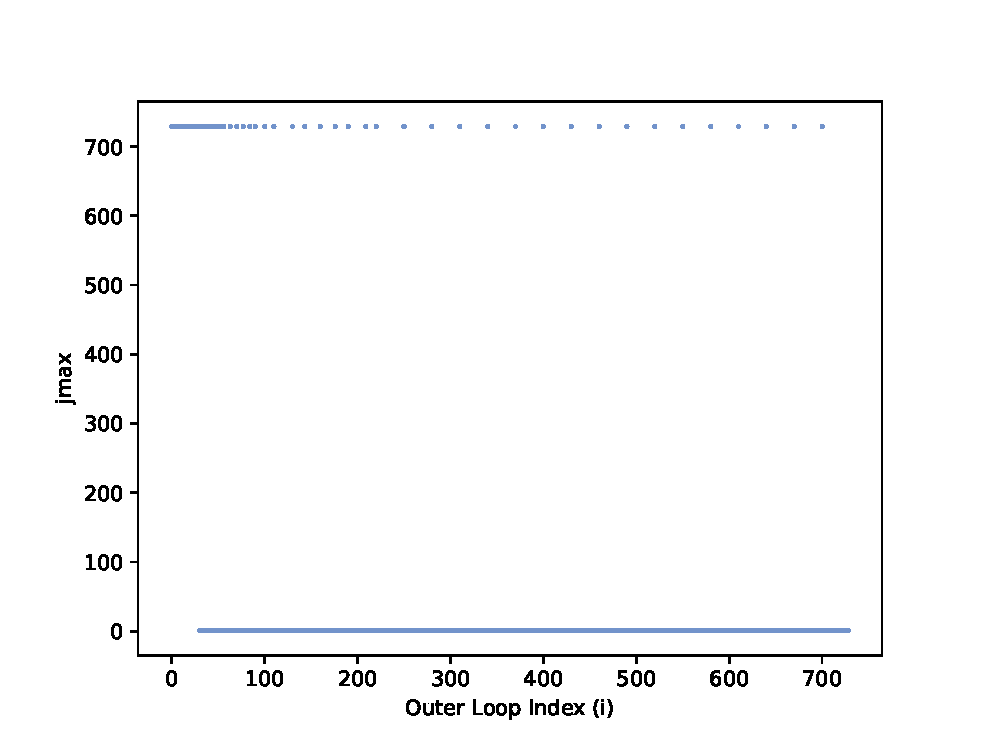
\includegraphics[scale=0.6]{../graphs/jmax.eps}
    \caption{Jmax value against Outer Loop Iteration in Loop 2}
    \label{jmax}
\end{figure}

In contrast, the affinity scheduling option is more scalable for the whole experiment but with tinier changes in running time. As we increase the number of threads when the latest of them finish with their Local Set, more are available to contribute calculation the first heavyweight iterations.

To sum up, the basic difference between these two scheduling options is that the affinity is able to redistribute heavy workload to other threads with a variety of Chunksize but dynamic is bound to calculate 16 iterations each time which is not optional for each of the threads configurations.

\subsubsection{Speedup}

According to Figure \ref{speedupLoop2}, comparing the speedup of affinity scheduling with the ideal, affinity seems to scale well. As we increase the number of threads, Chunksizes become smaller so the workload is easier to be distributed among the threads.

\begin{figure}[ht]
	\centering
	\includegraphics[scale=0.6]{../graphs/loop2_speedup.eps}
	\caption{Speedup Loop 2}
	\label{speedupLoop2}
\end{figure}

The trend changes when we move from 12 to 16 threads. Using 12 threads the heaviest Local Set is the first one containing exactly 729 (iterations) / 12 (number of threads) = 60 iterations. This means that it will possibly be the thread with the slowest progress, so each other will try to steal from it. The issue is that when we use 16 threads then each Local Set will have 729 / 16 = 45 iterations. As results the heavy workload will be distributed among thread 1 and 2. Keeping in mind that being the most loaded thread doesn't mean you have the most intense calculations. Then an issue occurs, because the other threads will try to steal with a greater possibility from other than thread 1 and 2. This leads to an unfair balance distribution.

In terms of dynamic, 16 scheduling, it is plain to see that if we use more than 6 threads, its speedup is constant. This happens because adding more threads after that point has no overall effect due to the fact that there are no additional heavy calculations. The first thread will have been assigned with the heavy workload, and the remaining will be underutilized.

\sectionVspacing

\section{Conclusion}
In conclusion, the affinity scheduling option is optimal for loops that the workload is equally distributed in different iterations. If this not the case, lightweight threads can steal workload from the heavyweight Local Sets which is a good load balancing approach. As we approach the end of the loop this happens to be the bottleneck because the Chunks become smaller. Giving an option to the scheduler for the smallest Chunksize could solve this problem reducing redundant race conditions between the threads.

\end{document}
